\chapter{Case Study}
\label{chapter3}
For this project, a case study focused on taking a closer look into the popular XCUITest test automation framework and other XCTest based user interface test automation frameworks will be performed. In order to achieve this, an iOS application, a set of test cases and automated tests are needed.


\section{Firefox iOS App}
After exploring several open source applications, the Firefox project for iOS seemed to be the best fit, since it provides a big enough and stable application as well as hundreds of working automated UI tests. These automated tests make use of the XCUITest framework for black box testing along with KIF and EarlGrey for grey box testing. On the other hand, the project is currently up to date regarding the software versions used and it is constantly been worked on, which greatly reduces compatibility issues. \cite{FirefoxAppiOS}

\section{Test Cases}
Considering the objective of this case study is to compare the different test automation tools, the following set of test cases aims to cover as many different situations one could encounter while testing, and not providing a coverage for the application itself. This means, they will try to cover as many of the GUI components, gestures and testing capabilities as possible within the existing automated tests in the Firefox App.

\subsection{XCTestUI Test Cases}
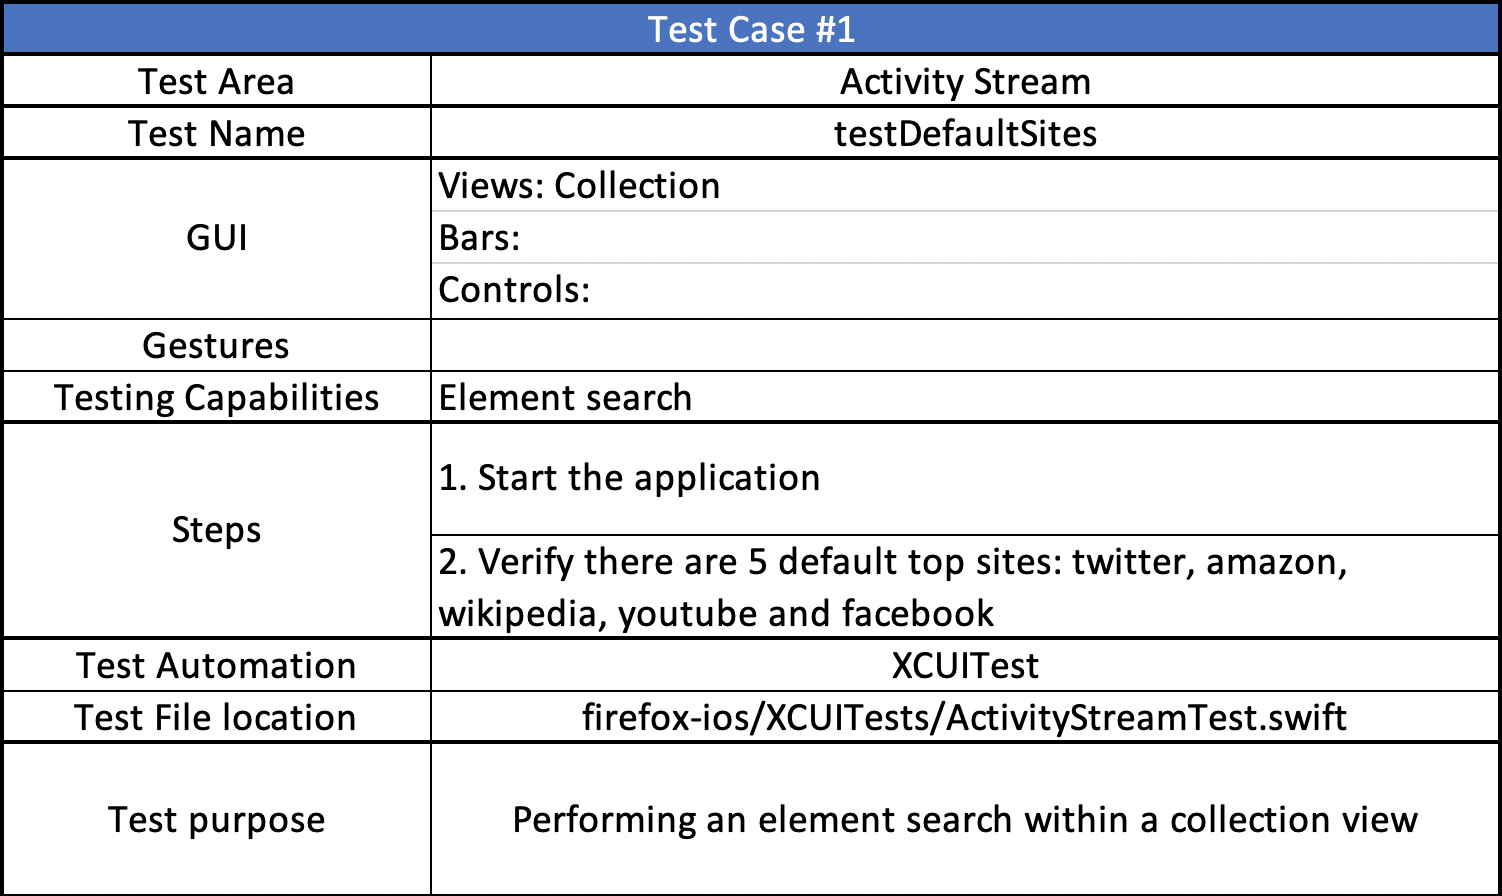
\includegraphics[width=10cm]{img/tc1.png} \\[2mm]
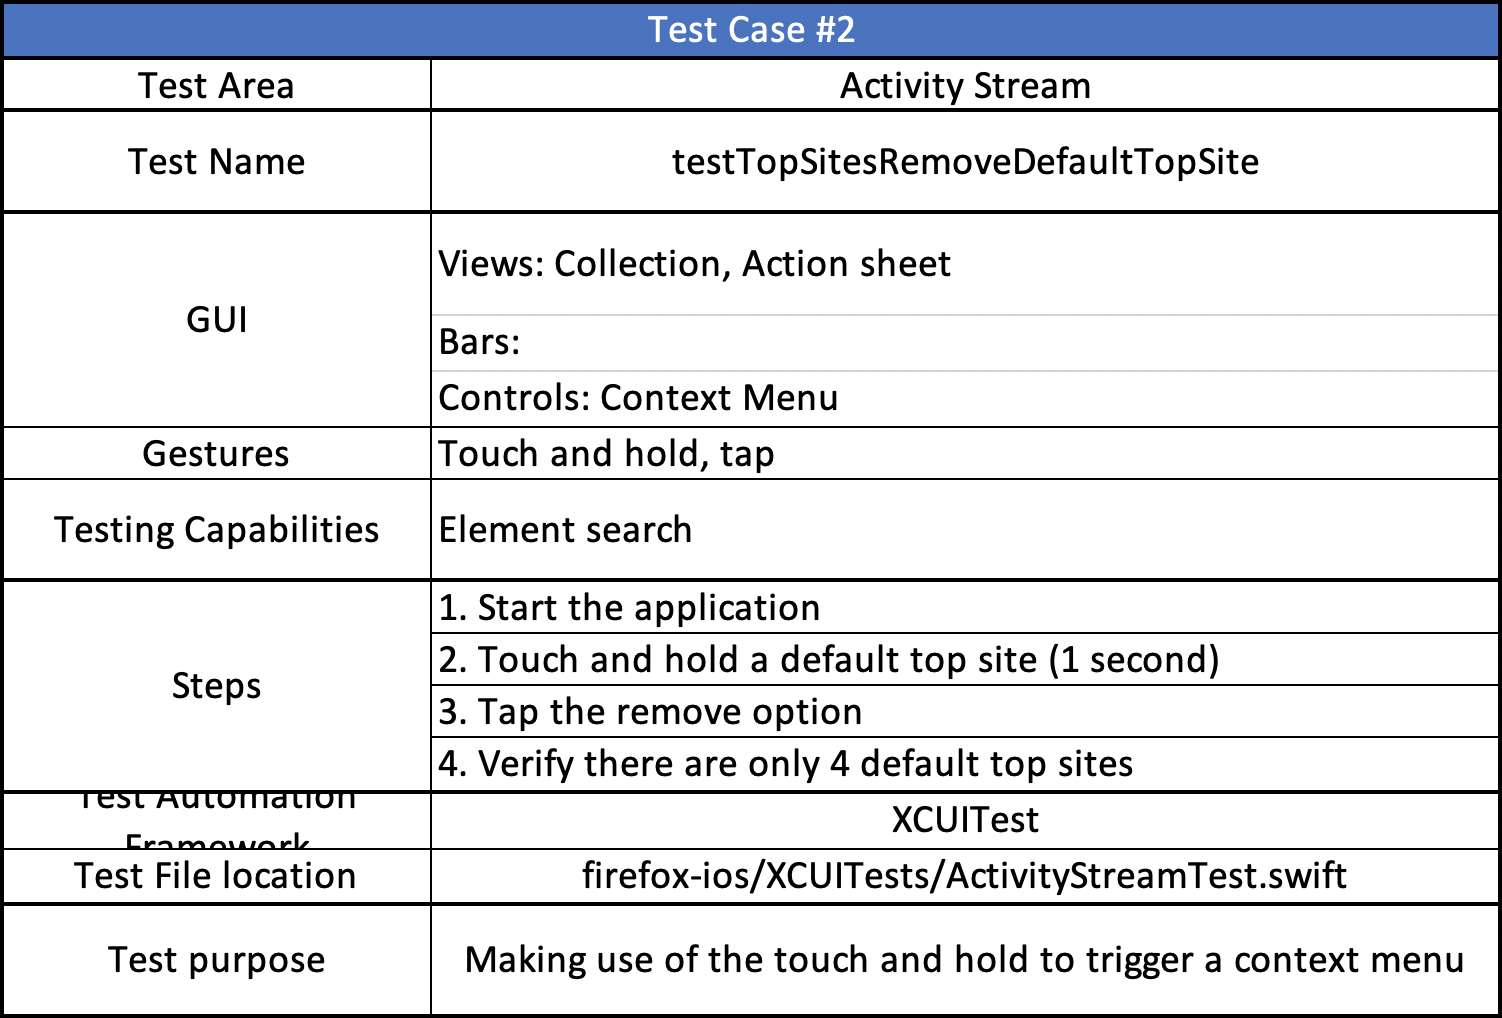
\includegraphics[width=10cm]{img/tc2.png} \\[2mm]
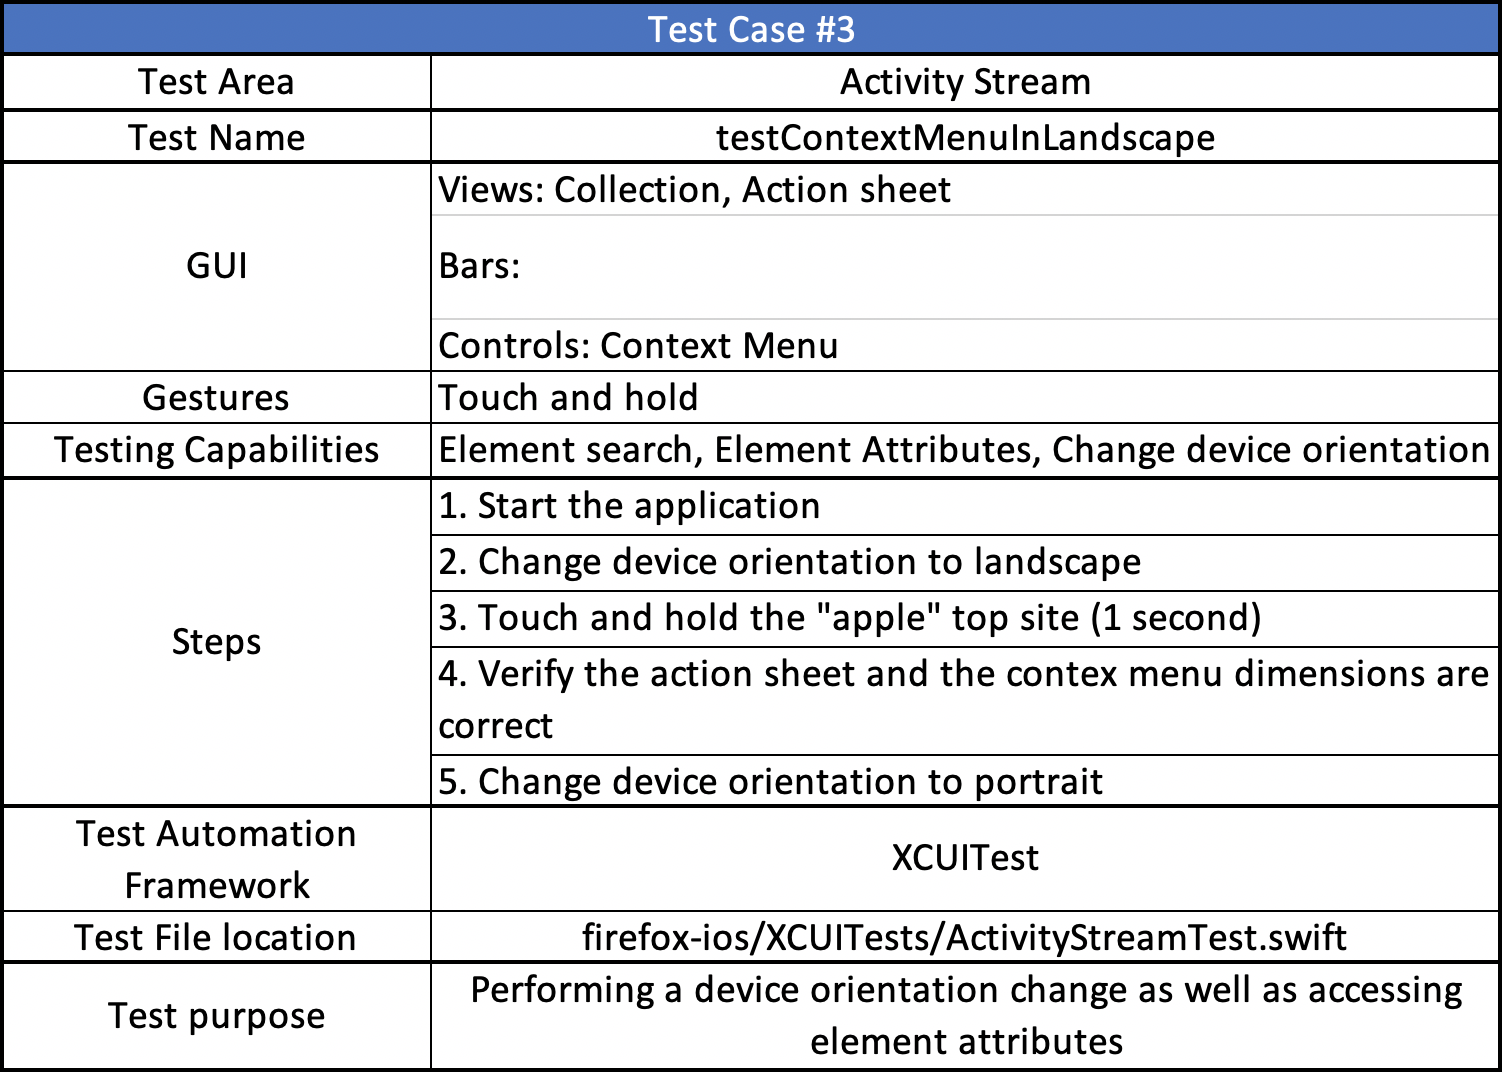
\includegraphics[width=10cm]{img/tc3.png} \\[2mm]
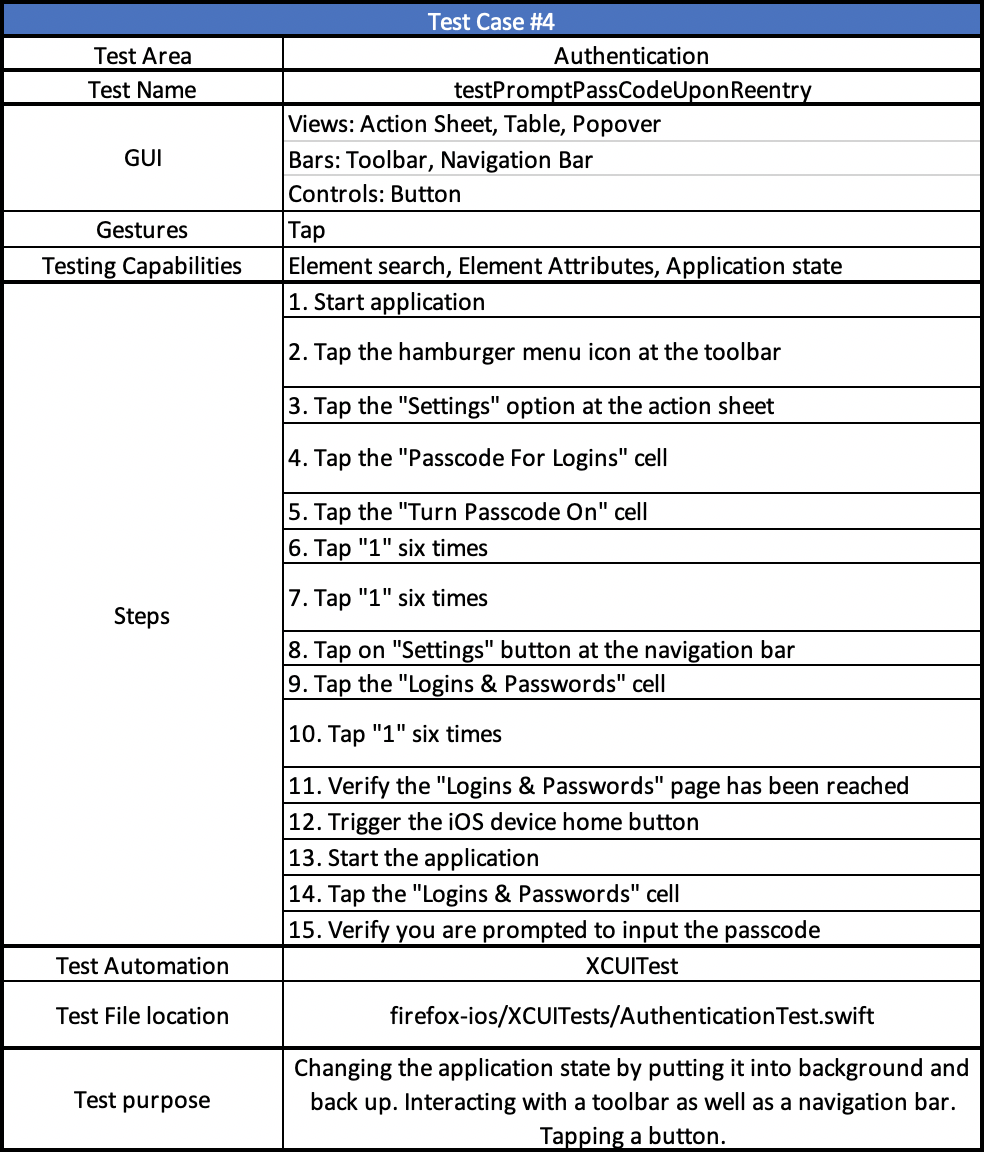
\includegraphics[width=10cm]{img/tc4.png} \\[2mm]
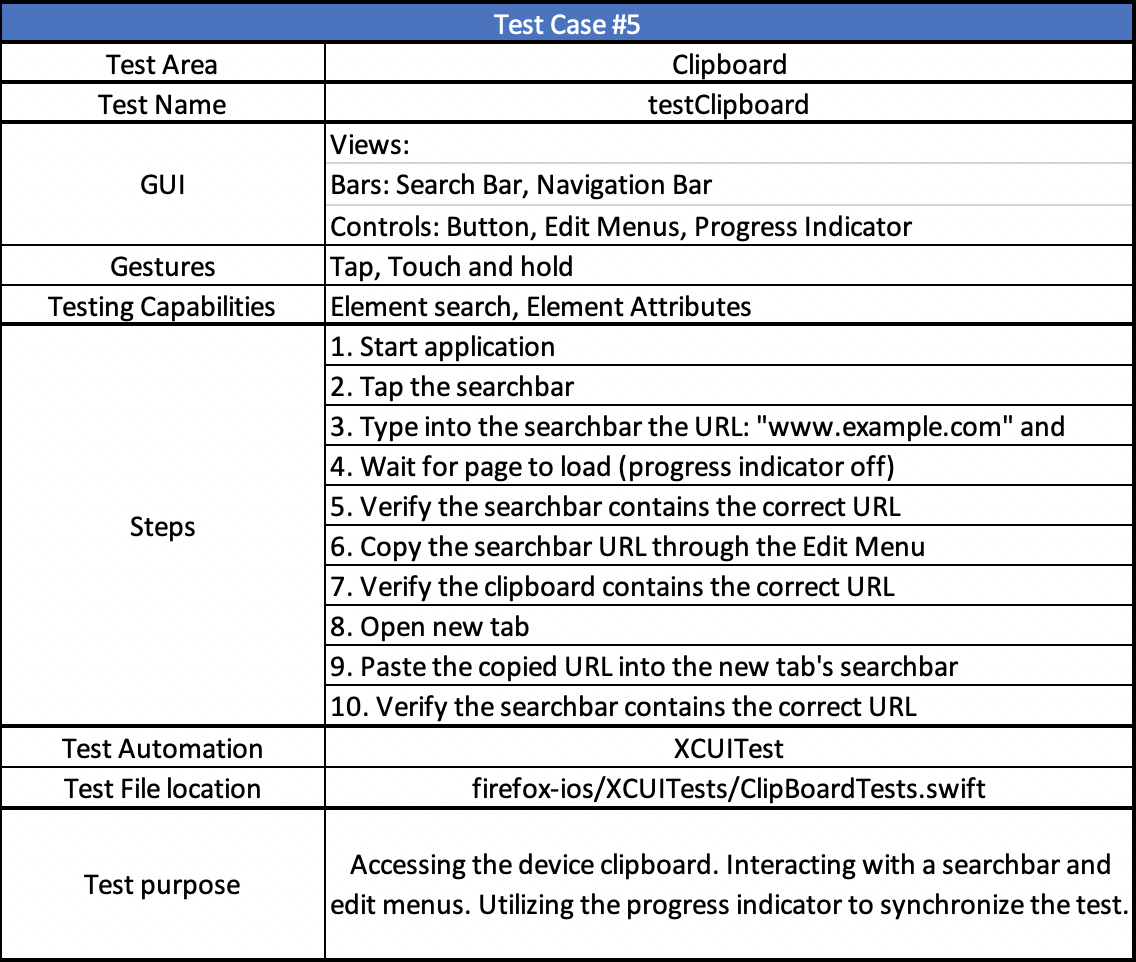
\includegraphics[width=10cm]{img/tc5.png} \\[2mm]
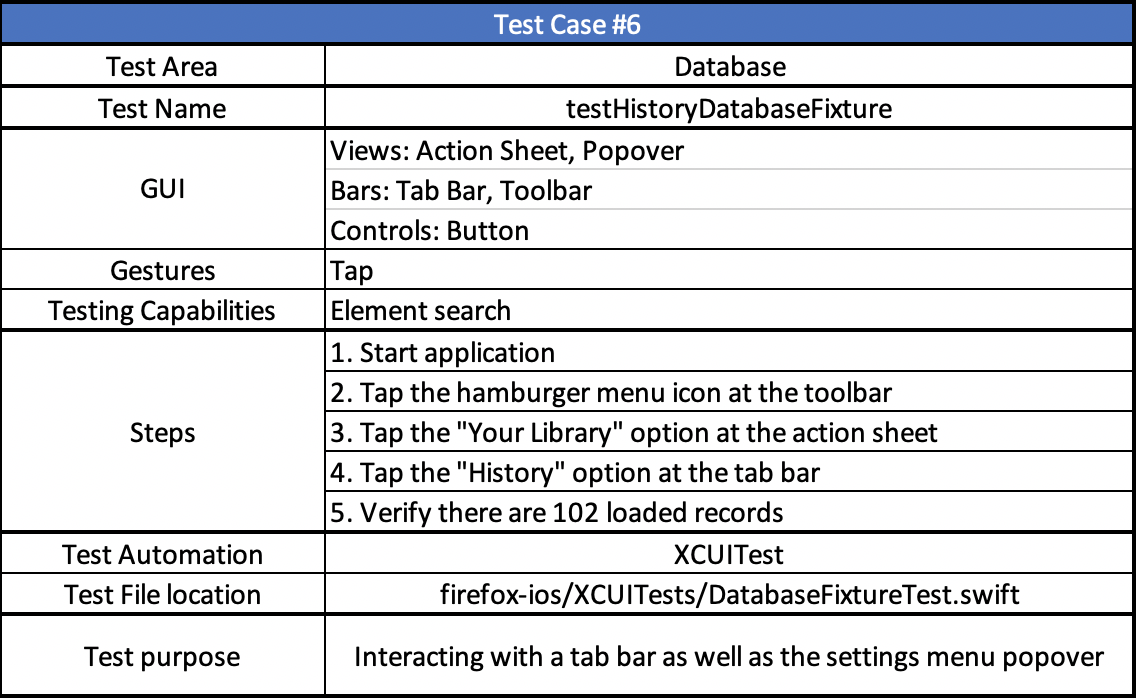
\includegraphics[width=12cm]{img/tc6.png} \\[2mm]
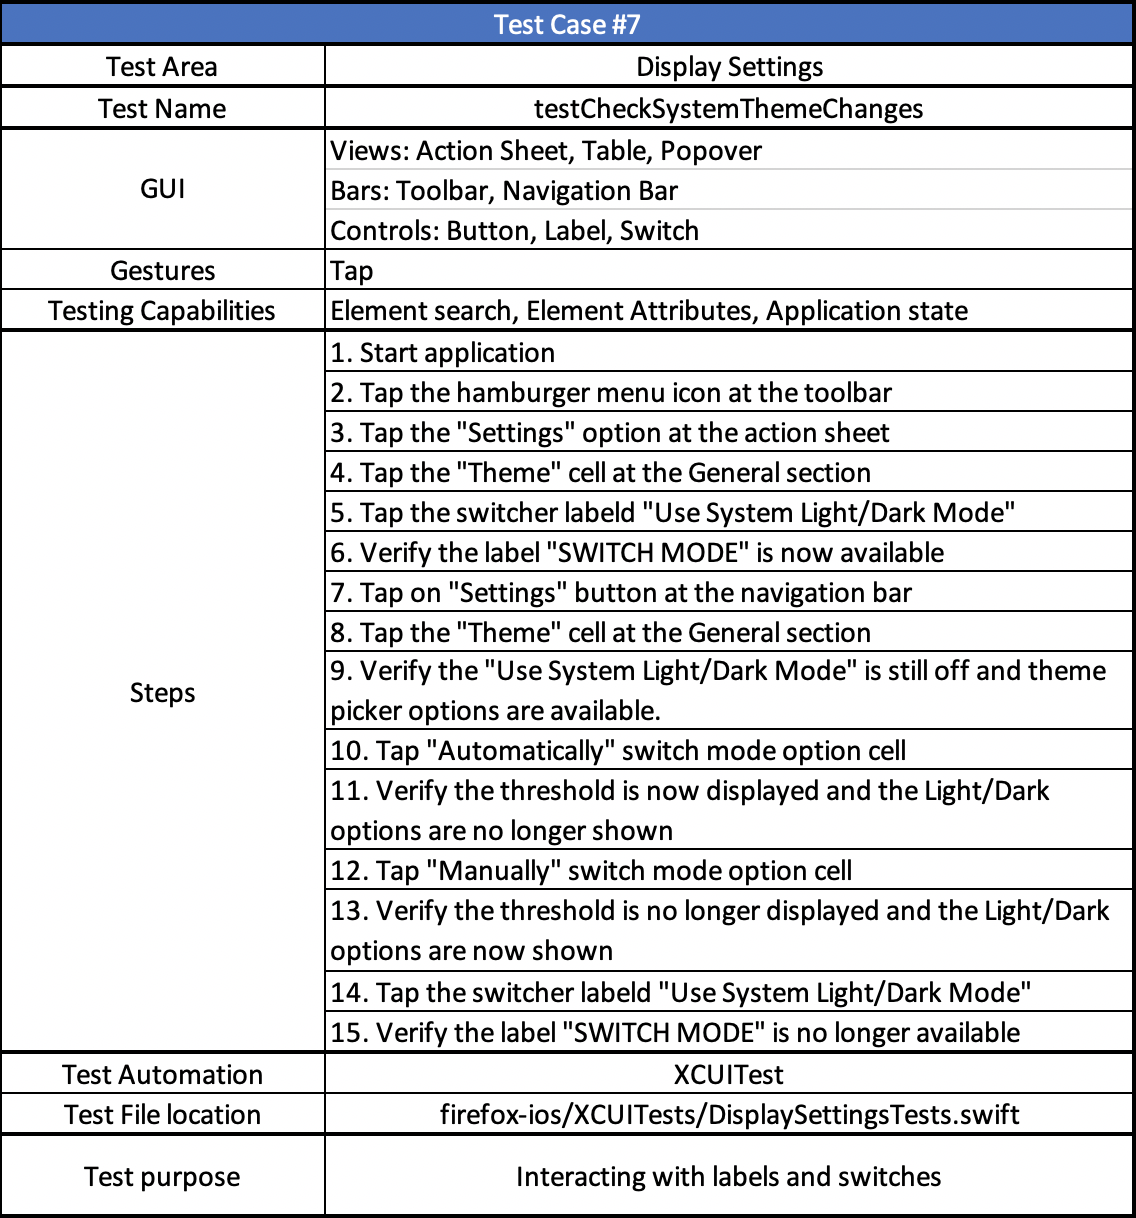
\includegraphics[width=12cm]{img/tc7.png} \\[2mm]
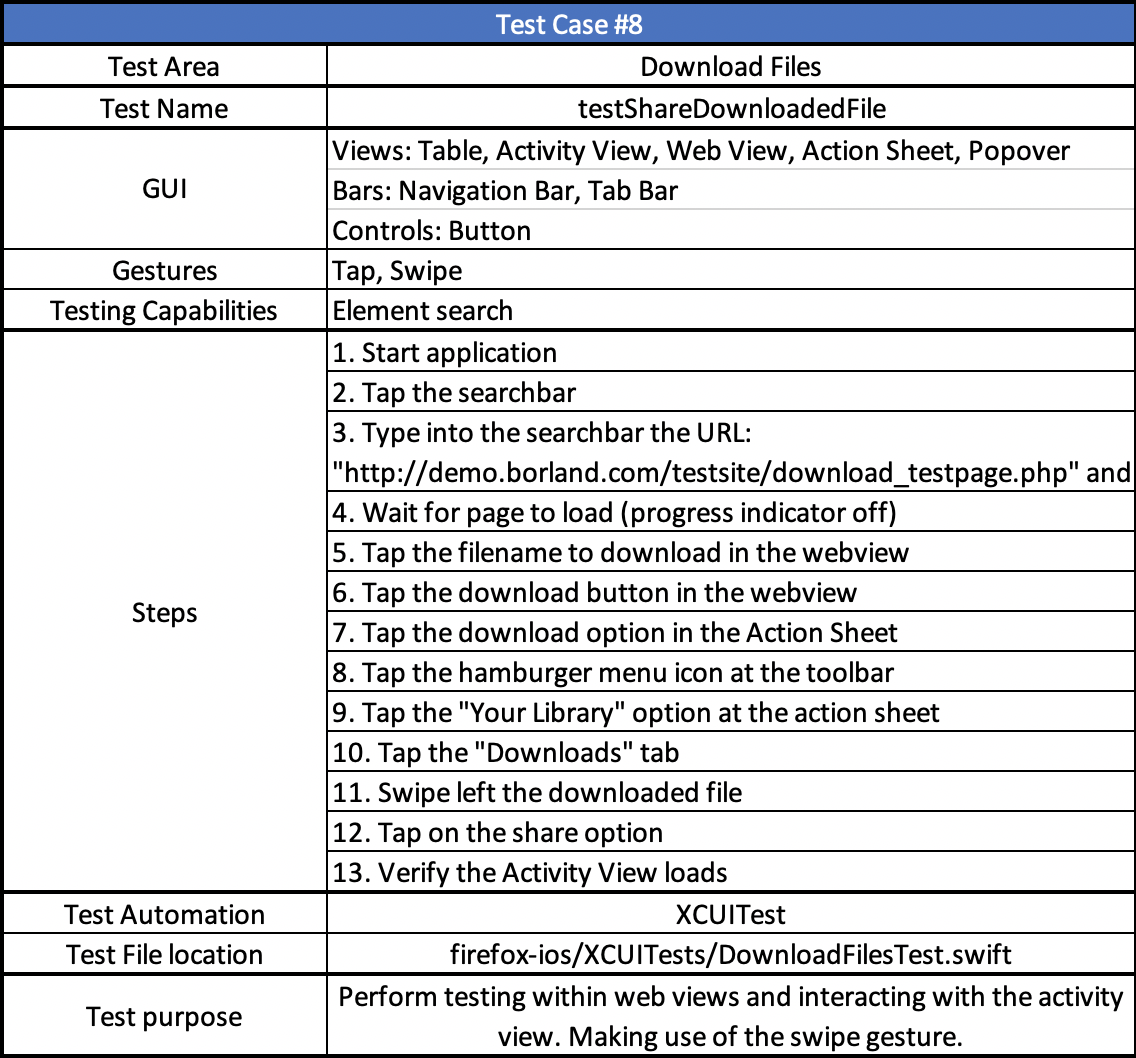
\includegraphics[width=12cm]{img/tc8.png} \\[2mm]
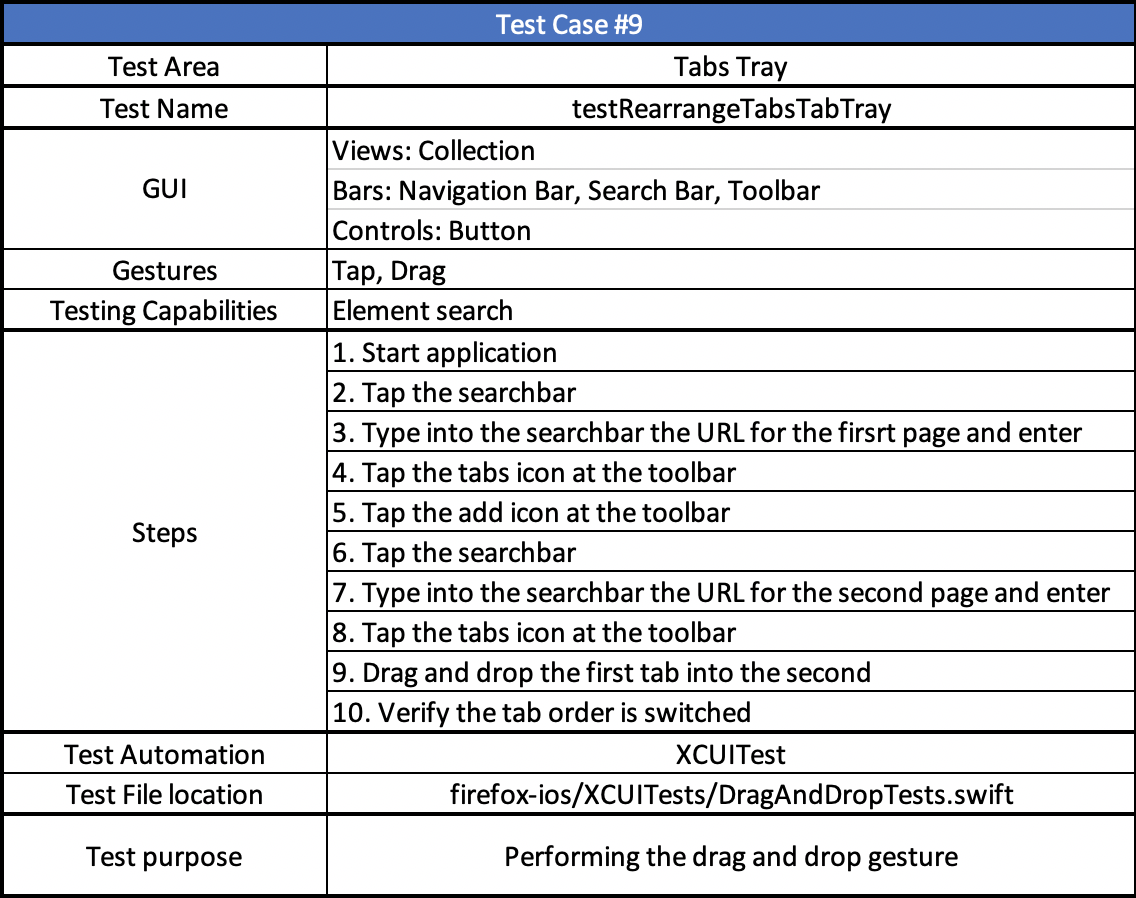
\includegraphics[width=12cm]{img/tc9.png} \\[2mm]
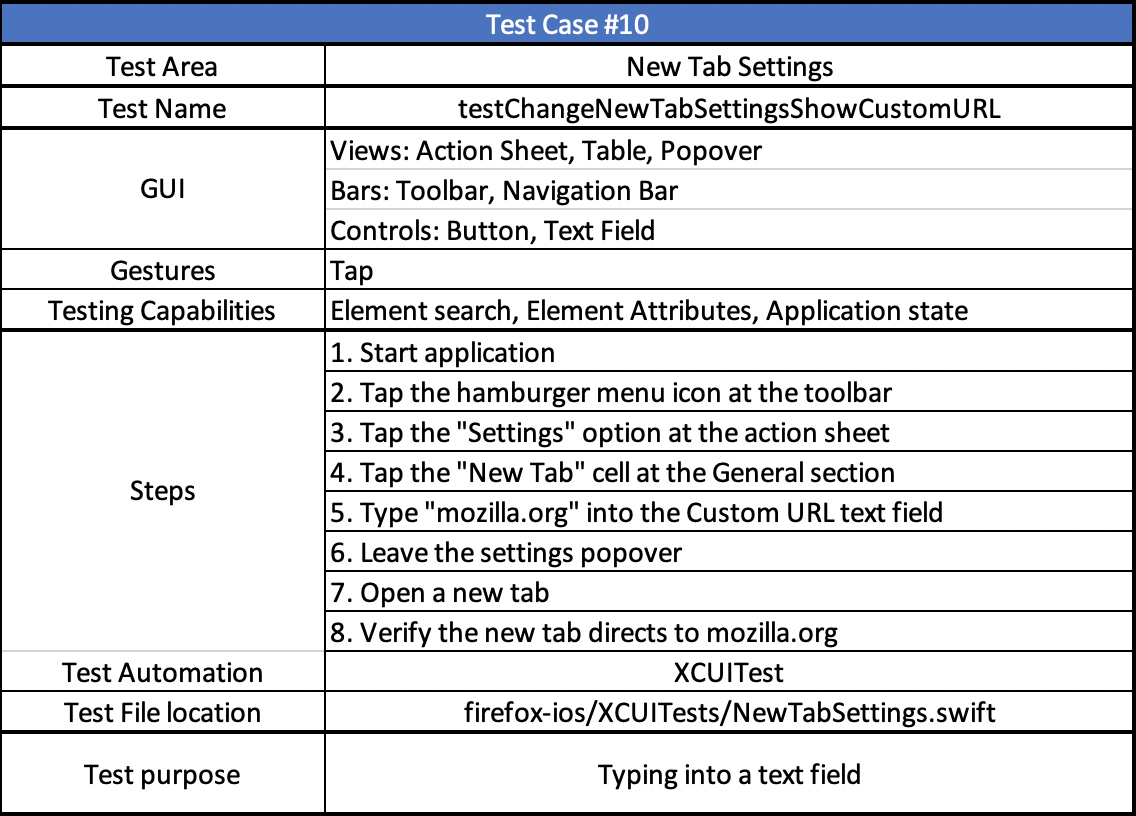
\includegraphics[width=12cm]{img/tc10.png} \\[2mm]

\subsection{KIF and EarlGrey Test Cases}
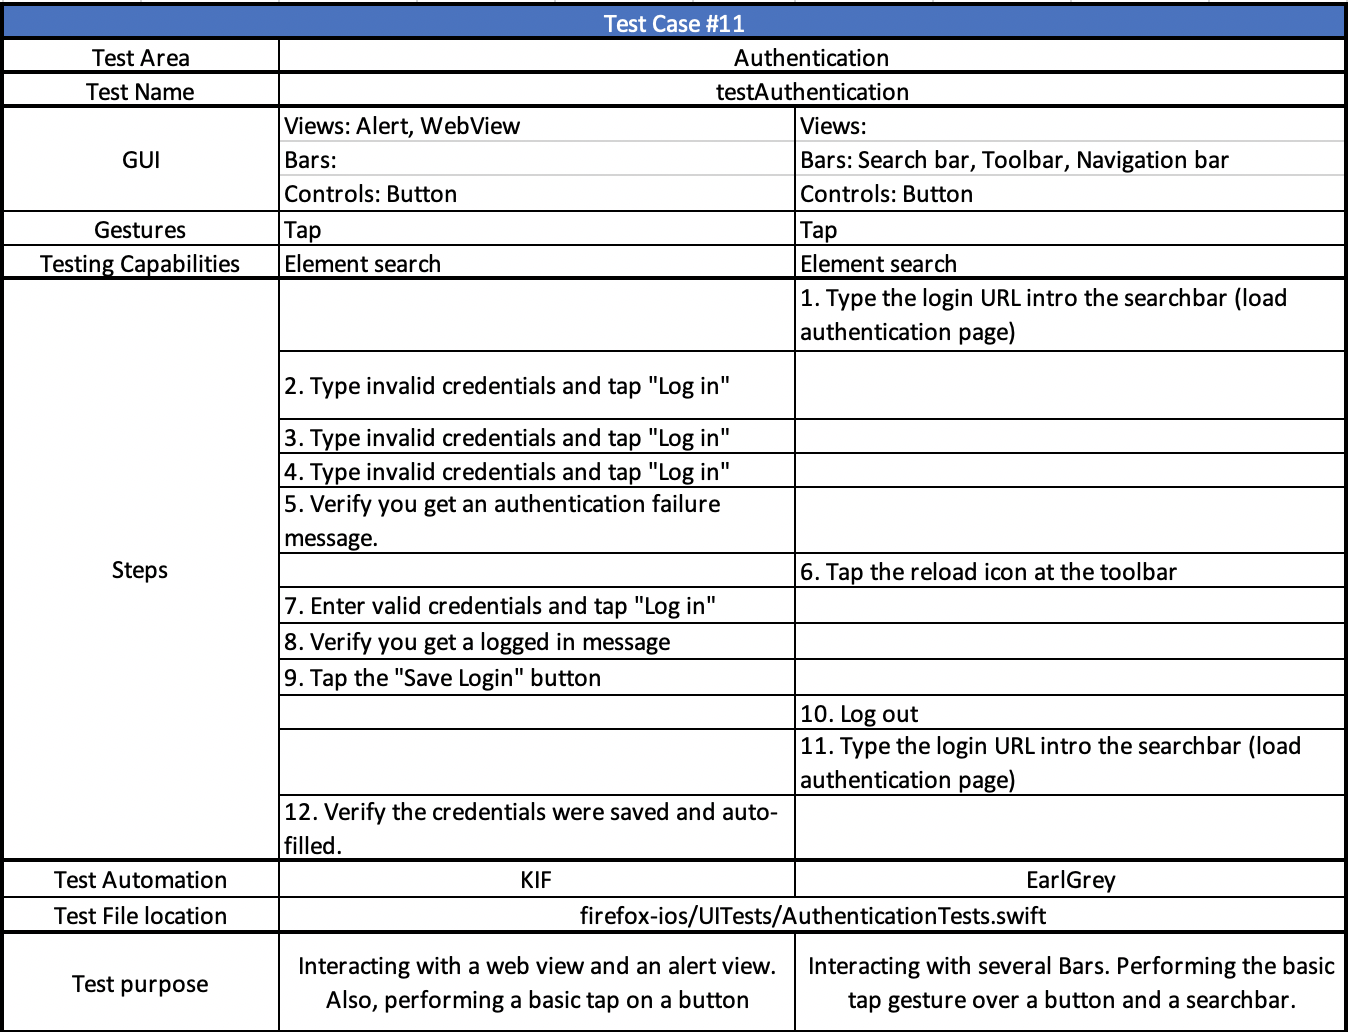
\includegraphics[width=12cm]{img/tc11.png} \\[2mm]
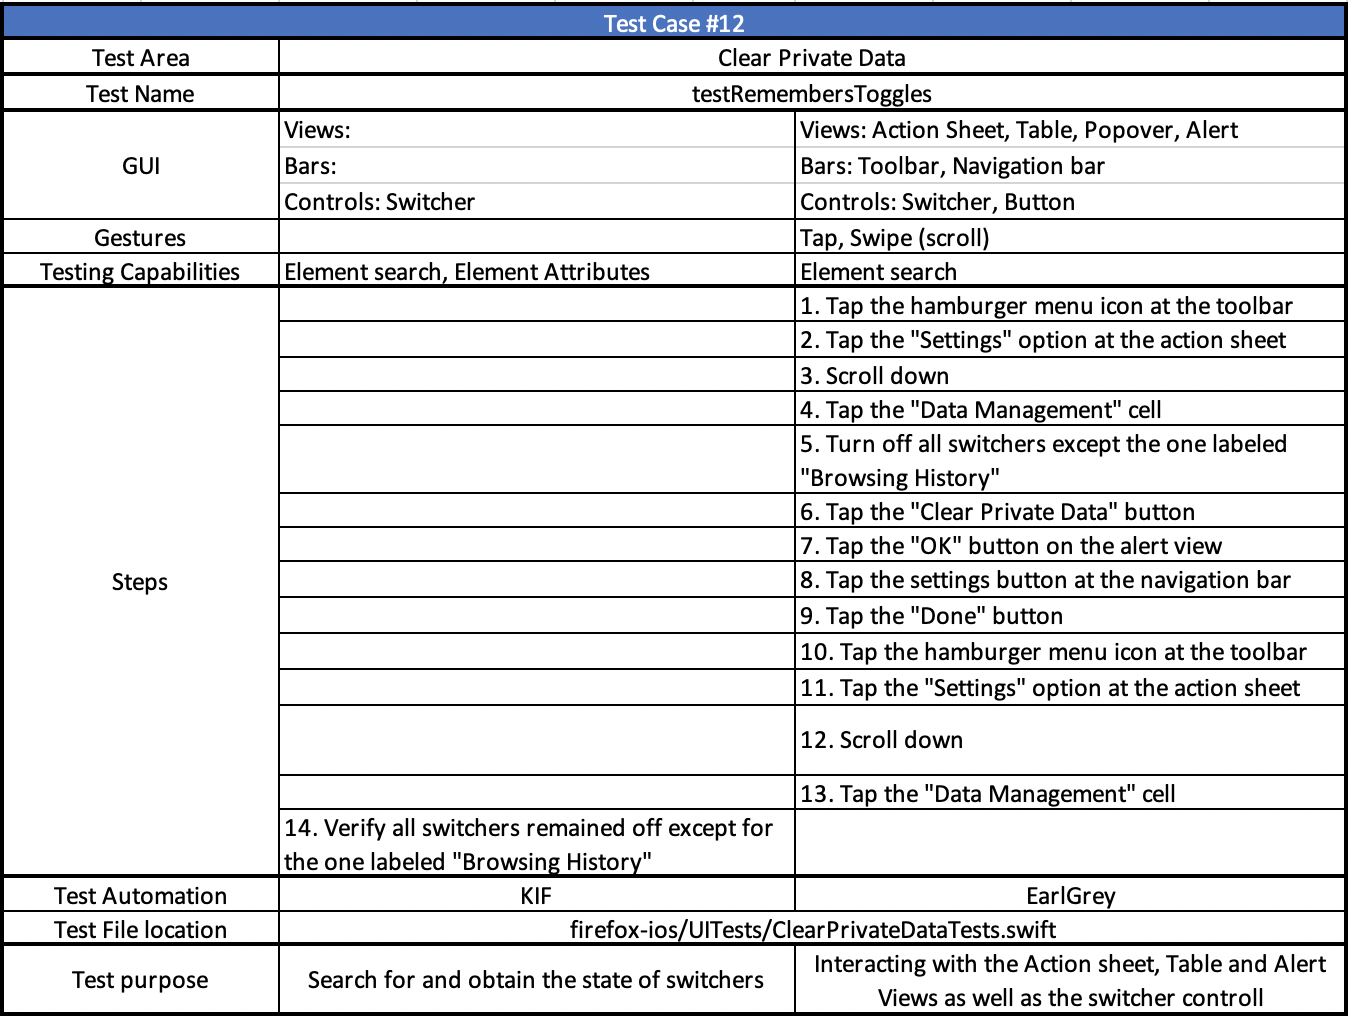
\includegraphics[width=12cm]{img/tc12.png} \\[2mm]
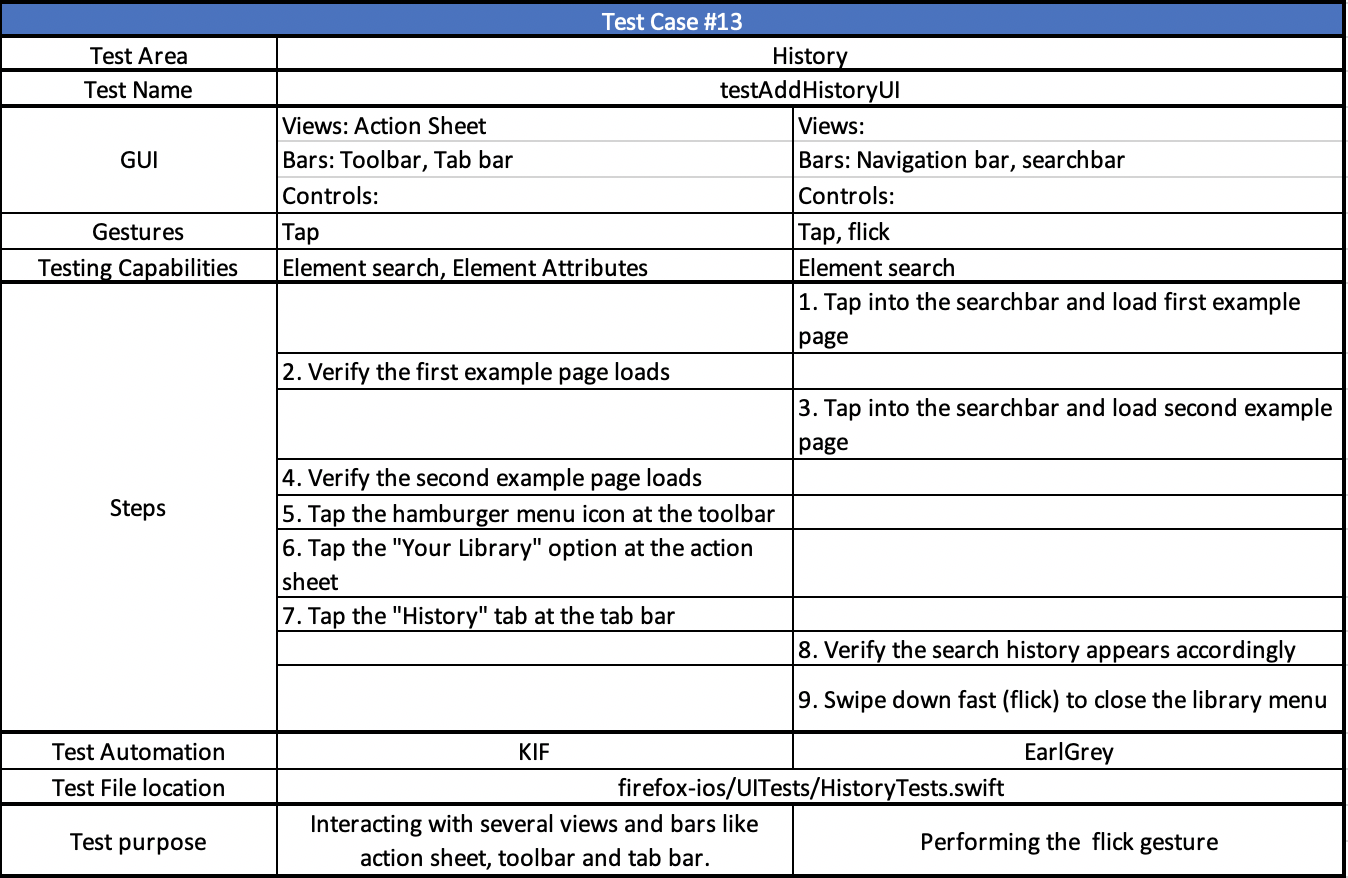
\includegraphics[width=12cm]{img/tc13.png} \\[2mm]

\section{Results}
The following tables provide, for each tool, a view which matches a specific GUI component, gesture or testing capability with a test case that involves it. This is particularly useful if you desire to explore a real-world example of an automated UI test for some of the different GUI components, gestures and framework testing capabilities or to check out the coverage of the tool.


	\subsection{XCTestUI}
	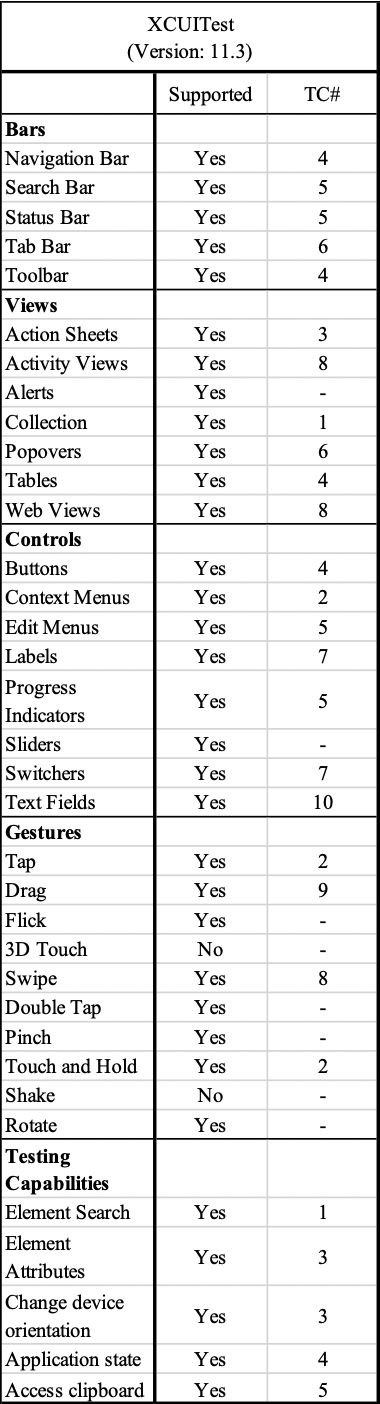
\includegraphics[width=5.5cm]{img/table2.png} \\[2mm]
	
	\subsection{KIF}
	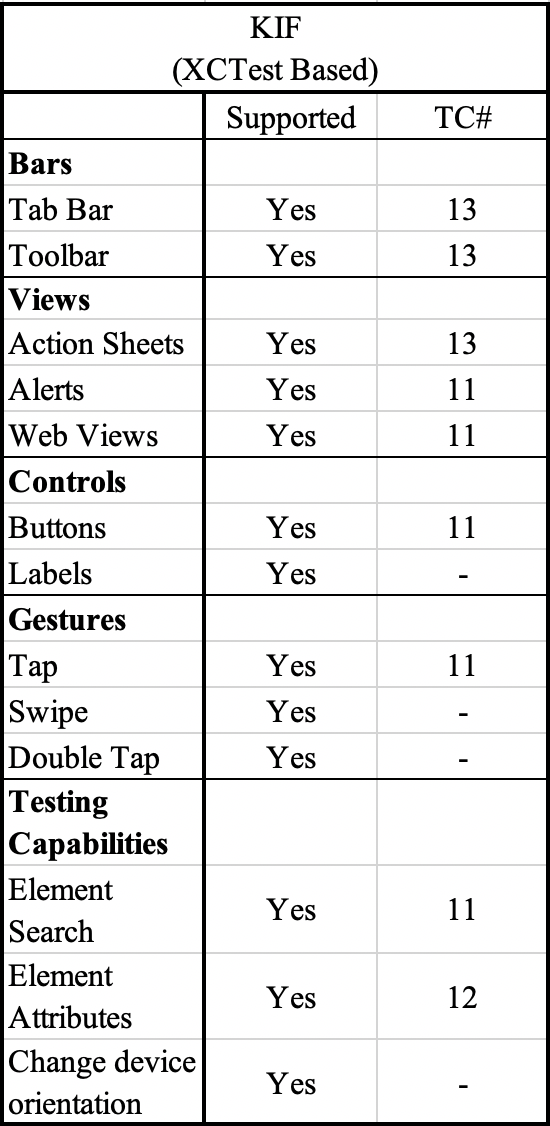
\includegraphics[width=10cm]{img/table3.png} \\[2mm]

	\subsection{EarlGrey}
	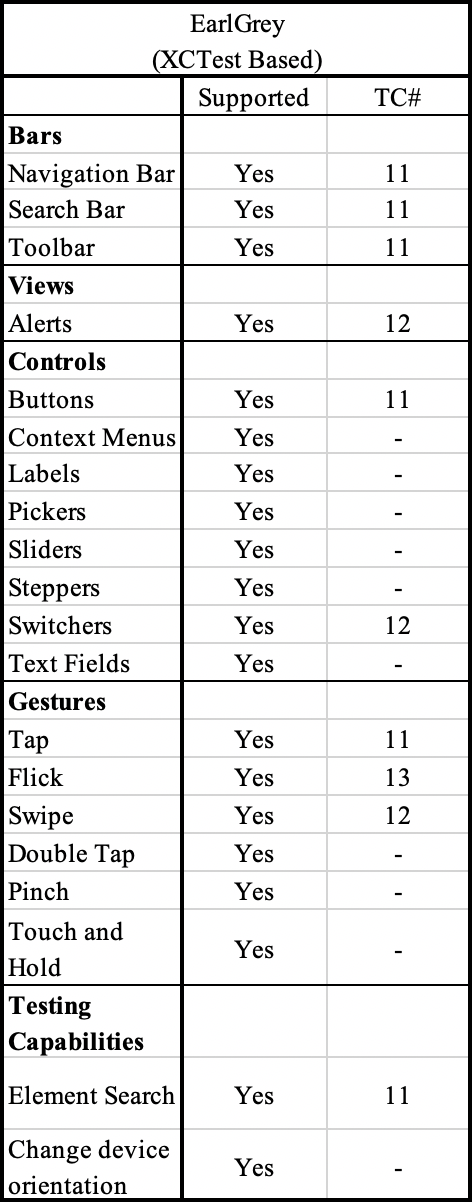
\includegraphics[width=6cm]{img/table4.png} \\[2mm]

After some extra research, the coverage of several GUI components, gestures and framework testing capabilities could be exhibited. However, these do not have a related test case as there is no automated test in the Firefox App to associate them with. It is also important to take into account the fact that not all GUI components, gestures and framework testing capabilities were evaluated.



	
